\documentclass[../sparc.tex]{subfiles}
\graphicspath{{\subfix{../images/}}}
\begin{document}

%%%%%%%%%%%%%%%%%%%%%%%%%%%%%%%%%%%%%%%%%%%%%%%%%%%%%%%%%%%%%%%%%%%%%%%%%%%%%%%%
\section{Resistance}
\label{section:electronics-resistance}
\index{Electronics!Resistance}

To be able to calculate the speed of the water flowing from one vessel to
another we have to know the parameters of the pipe that connecting the vessels --
in the other words, the parameters of the \emph{water conductor}.  And one of
the main parameter is the \emph{resistance} of the pipe.  The greater the
resistance, the slower the water will flow.

We can use a pipe with a small inner diameter as an example of water conductor
with high resistance, as shown on fig. \ref{fig:electronics-resistance-0}.

\begin{figure}[ht]
  \centering
  \def\offset{6}
  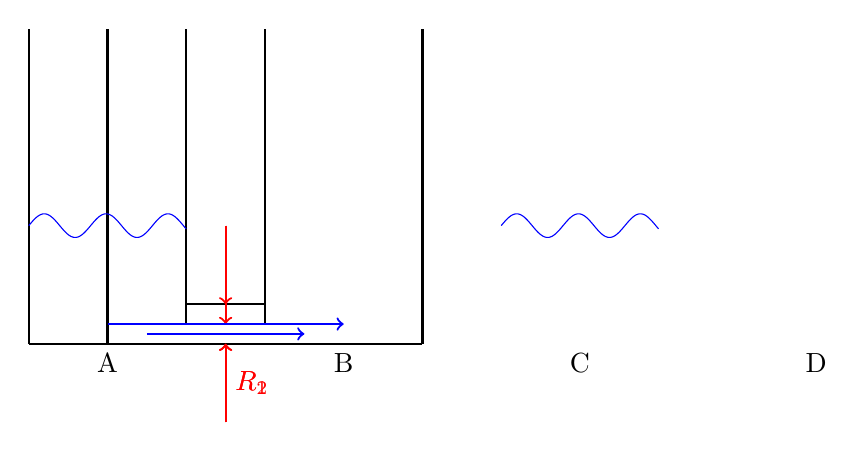
\begin{tikzpicture}[
      declare function={f1(\x) = 0.15 * sin(8.0 * deg(\x));
    }]

    \draw[thick] (0, 0) -- (0, 4);
    \draw[thick] (2, 0.5) -- (2, 4);
    \draw[thick] (0, 0) -- (2, 0);

    \draw[thick] (3, 0.5) -- (3, 4);
    \draw[thick] (5, 0) -- (5, 4);
    \draw[thick] (3, 0) -- (5, 0);

    \draw[thick] (2, 0) -- (3, 0);
    \draw[thick] (2, 0.5) -- (3, 0.5);

    \draw[thick] (\offset, 0) -- (\offset, 4);
    \draw[thick] (\offset + 2, 0.25) -- (\offset + 2, 4);
    \draw[thick] (\offset, 0) -- (\offset + 2, 0);

    \draw[thick] (\offset + 3, 0.25) -- (\offset + 3, 4);
    \draw[thick] (\offset + 5, 0) -- (\offset + 5, 4);
    \draw[thick] (\offset + 3, 0) -- (\offset + 5, 0);

    \draw[thick] (\offset + 2, 0) -- (\offset + 3, 0);
    \draw[thick] (\offset + 2, 0.25) -- (\offset + 3, 0.25);

    \draw[thick, color=red, ->] (2.5, 1.5) -- (2.5, 0.5);
    \draw[thick, color=red, ->] (2.5, -1) -- (2.5, 0);
    \draw[color=red] (2.5, -0.5) node[right] {$R_1$};

    \draw[thick, color=red, ->] (\offset + 2.5, 1.5) -- (\offset + 2.5, 0.25);
    \draw[thick, color=red, ->] (\offset + 2.5, -1) -- (\offset + 2.5, 0);
    \draw[color=red] (\offset + 2.5, -0.5) node[right] {$R_2$};

    \draw[thick, color=blue, ->] (1, 0.25) -- (4, 0.25);

    \draw[thick, color=blue, ->] (\offset + 1.5, 0.125) -- (\offset + 3.5, 0.125);

    \begin{scope}[yshift=1.5cm, color=blue]
      \draw (0, 0) plot[domain=0:2, variable=\x, samples=200, smooth] ({\x}, {f1(\x)});
    \end{scope}

    \begin{scope}[yshift=1.5cm, xshift=6 cm, color=blue]
      \draw (0, 0) plot[domain=0:2, variable=\x, samples=200, smooth] ({\x}, {f1(\x)});
    \end{scope}

    \draw (1, 0) node[below] {A};
    \draw (4, 0) node[below] {B};
    \draw (7, 0) node[below] {C};
    \draw (10, 0) node[below] {D};

  \end{tikzpicture}
  \caption{An example of two vessels connected with pipes with different
    resistance to the water flow.}
  \label{fig:electronics-resistance-0}
\end{figure}

The smaller the inner diameter of a pipe, the higher the resistance.  The same
rule can be applied to an electric conductor (e.g. a piece of wire) where the
diameter of a wire and its resistance have inverse relationship: the thicker the
wire the lesser its resistance to the electric current.  Thus the lesser the
resistance the greater the electric current.

Let's assume that the vessel ``B'' and the vessel ``C'' on
fig. \ref{fig:electronics-resistance-0} are connected with a pipe with one-half
of the pipe diameter that connects vessels ``A'' and ``B''.  Then the water
current between vessels ``B'' and ``C'' will be two times smaller than the water
current between vessels ``A'' and ``B''.

In the electronics we measure the resistance of a conductor in Ohms.

The relationship between current, voltage and resistance is described in
\emph{Ohms Law}.  Using this law we can calculate the electric current for an
electric circuit, using formulae \ref{equation:elemctronics-ohms-law-0}.

\begin{equation}
  \mbox{I} = \frac{\mbox{U}}{\mbox{R}}
  \label{equation:elemctronics-ohms-law-0}
\end{equation}

Where ``I'' is the current (in Amperes), ``U'' is the voltage (in Volts) and
``R'' is resistance (in Ohms.)

In day-to-day life we can be pretty sure that any wire or a piece of some
conducting material (e.g. metal) has some non-zero resistance.  Some materials
have greater resistance than the others.  Such materials that have low
resistance called \emph{conductors}.  Copper, silver and gold are examples of
good conductors.  Materials that have high resistance commonly used as
\emph{insulator} and they are called \emph{dielectric}.  We can put in this
category different kinds of plastics that are used as the material for wire
insulators.

\experiment{0}{Look around you -- how many conductors can you find?}

When electric current flows through a conductor that has some resistance (that
is, through any common conductive material) some percentage of the energy get
lost by turning into heat radiated from the conductor.  For example when you
plug an electric kettle into a power socket and turn it on, not only the kettle
heater gets hot, but the wires that conduct the electricity from the wall socket
to the kettle.  Although the heating of wires is miniscule in comparison the the
temperature of the water heater inside the kettle.

In some cases the heating of a conductor is the desired effect itself as in the
case of an electric kettle; in other cases engineers try to lower the resistance
of a conductor that in turn lower the heating -- because the heating is but an
energy loss and is unwanted.

\end{document}
